\chapter{Resultat}

I detta kapitel redovisas kortfattat det resulterande läromaterialet, vilket består av fem kapitel. Det är även publicerat på en hemsida och dess källkod är fritt tillgänglig. Även
resultaten från utvärderingen med testgruppen och mötena med Åke Fäldt redovisas.

\section{Läromaterialet}\label{sec:res_laromaterial}

Läromaterialet blev till slut en sammanvävning av domänspecifika språk som
modellerar fysik, och en lärotext som förklarar kopplingen mellan fysiken och de
domänspecifika språken. Figur~\ref{fig:smakprov_laromaterial} visar ett kort
utdrag ur läromaterialet. Där ses hur domänspecifika språk och lärotext
är sammanvävda. Ett längre utdrag finns i bilaga~\ref{cha:utdrag}.

\begin{figure}[tph]
  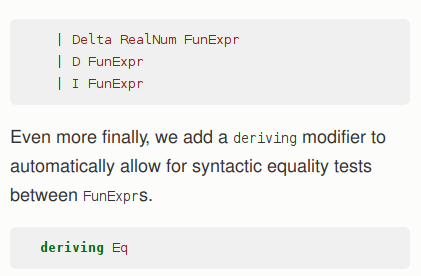
\includegraphics[width=\linewidth]{figure/smakprov_laromaterial.png}
  \caption{Ett smakprov av det resulterande läromaterialet. Lärotexten ligger mot den ljusgrå bakgrunden medan det domänspecifika språket ligger mot den mörkgrå. Notera att detta exemplets källkod (i Litterate Haskell) har visats tidigare i avsnitt \ref{sec:lhs}.}~\label{fig:smakprov_laromaterial}
\end{figure}

Språket i lärotexten är enligt projektgruppen lättsamt\footnote{Diskuteras utförligare i avsnitt \ref{sec:res_disk}.} och det finns även bilder och övningar.
Figur~\ref{fig:smakprov_bild_laromaterial} är ett exempel på en bild ur
läromaterialet. Notera speciellt den medvetet oseriösa ritningstekniken som är
tänkt att vara rolig och muntra upp läsaren. Övningar ligger både i den löpande
texten och i slutet av kapitlet. Övningarna i den löpande texten innebär oftast
att läsaren ska implementera en liten del av det aktuella domänspecifika språket
på egen hand, vilket illustreras i figur~\ref{fig:smakprov_ovning}. Övningarna i slutet av kapitlet innebär ofta större vidareutvecklingsmöjligheter av de domänspecifika språken.

\begin{figure}[tph]
    \centering
    \begin{subfigure}[t]{0.5\textwidth}
        \centering
        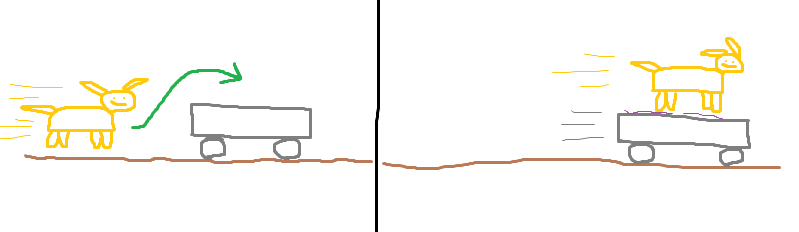
\includegraphics[width=0.9\linewidth]{figure/smakprov_bild_laromaterial.png}
        \caption{Exempel på en bild. Bilden visar hur en hund springer och
                 hoppar upp på en stillastående
                 vagn.}~\label{fig:smakprov_bild_laromaterial}
    \end{subfigure}%
    ~~~
    \begin{subfigure}[t]{0.5\textwidth}
        \centering
        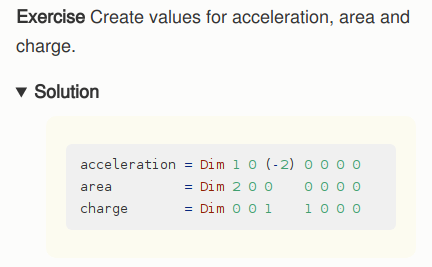
\includegraphics[width=0.9\linewidth]{figure/smakprov_ovning.png}
        \caption{Exempel på en övning. Övningen ligger som en del av den
                 löpande texten.}~\label{fig:smakprov_ovning}
    \end{subfigure}
    \caption{Exempel på en bild och en övning ur läromaterialet.}
\end{figure}

Läromaterialet behandlar ett flertal områden inom fysik och matematik.
Fokuset är på klassisk mekanik samt den matematik som tillhör området. I
sin fullständighet är de behandlade områdena:

\begin{itemize}
  \item Dimensioner
  \item Matematisk analys
  \item Vektorer
  \item Exempelproblem
  \item Partikelmekanik
\end{itemize}

\textit{Dimensioner} behandlar fysikaliska dimensioner, storheter och enheter inom fysiken.
Fysikaliska dimensioner införs på typnivå i Haskell för att visa likheten mellan
Haskells typsystem och hur dimensioner hanteras inom fysiken.
Typnivåprogrammering\footnote{Vanligtvis manipuleras \textit{värden} när
programmerering sker i Haskell och andra språk. Typnivåprogrammering är precis som
vanlig programmering med skillnaden att den sker på typnivån, det vill säga, att
typer modifieras. Läromaterialet~\cite{LYAP} hänvisas till för en utförligare
förklaring.} används för att göra likheterna så tydliga som möjligt.

I \textit{matematisk analys} behandlas differentialkalkyl och
integralkalkyl för en variabel. Först bestäms den semantiska domänen
för analys i en variabel: reella funktioner av ett argument; och ett syntaxträd
för uttryck av funktioner inom denna domän konstrueras. Därefter
analyseras syntax och semantik för differenser, derivator, och
integraler; och funktioner implementeras för att utföra dessa
operationer både approximativt numeriskt, och symboliskt med ett
syntaxträd. Slutligen appliceras de implementerade funktionerna för
att visualisera grafer av operationerna.

\textit{Vektorer} behandlar vektorer och vektoroperationer. Vektorer modelleras
med hjälp av en typklass som dikterar vilka funktioner som varje
modell av en vektor måste implementera. Generella vektoroperationer såsom
addition och skalärprodukt implementeras sedan med hjälp av dessa funktioner
vilket skapade ett mycket generellt och lättanvänt gränssnitt. QuickCheck
användes för att verifiera lagarna som gäller för olika vektoroperationer,
vilket gav en generell säkerhet kring att implementationerna var korrekta.

I \textit{exempelproblem} tillämpas de tre tidigare kapitlen på två vanliga mekanikproblem, nämligen \textit{krafter på lådor} och \textit{gungbräda}. I krafter på lådor används det domänspecifika språket för vektorer till att beräkna de krafter som verkar på en låda som glider ner för ett plan. I gungbräda visas hur momentjämviktsberäkningar kan göras med det domänspecifika språket för dimensioner.

\textit{Partikelmekanik}. En repetition av gymnasieskolans fysik.
Lägesenergi, rörelseenergi, gravitation och så vidare. Den modelleras med vektorer vars
komponenter består av matematiska uttryck tagna från kapitlet om matematisk
analys. Förhoppningen är att detta område inte ska presentera någon ny fysik för
läsaren utan istället visa hur redan känd fysik direkt går att översätta till
läromaterialets domänspecifika språk.

Läromaterialet blev publicerat på en hemsida~\cite{LYAP} och all källkod finns
tillgänglig på projektets GitHub~\cite{LYAP_repo}. På GitHub finns även ett
antal delvis färdigställda områden, till exempel bevisföring. Texten i
läromaterialet är skriven på engelska.

\section{Utvärderingen med testgruppen}\label{sec:res_test}

Utfallet från utvärderingen med testgruppen var till övervägande del positivt.
Testgruppen tyckte läromaterialet var ett intressant och roligt sätt att
presentera fysik på. De tyckte att bilderna tjänade sitt syfte i att muntra upp
läsaren.

En poäng som framfördes var att inte börja kapitlen för komplicerat. Istället
tyckte de att det skulle vara bra att börja enkelt, för att kunna hänga med i
både Haskell-koden och fysiken, och därefter behandla ett område mer
detaljerat. Att visa ett kort exempel i Haskell för att sedan låta läsaren själv
göra något liknande var ett förslag.

Utvärderingen var dock för kort för att det skulle framgå huruvida läsaren lärde
sig mest fysik eller mest Haskell. Det framgick heller inte om läromaterialet
uppmuntrade testgruppen att vilja lära sig mer fysik.

\section{Möten med fysikläraren}\label{sec:res_ake}

Åke Fäldt hade en överlag positiv syn på läromaterialet\footnote{Det bör
påpekas att det som är återgivet här självklart är en egen tolkning, och kan ha
missuppfattats, av projektgruppen. Fäldt ska med andra ord inte behöva stå till
svars för vad som står här.}. Fäldt tyckte att det fanns flera saker
läromaterialet kunde bidra med. En av dessa var att läromaterialet ger ett annat
perspektiv på fysiken, ett annat sätt att förklara den med
hjälp av domänspecifika språk. En annan sak var den rigorösitet som
domänspecifika språk leder till, eftersom de domänspecifika språken måste vara
väldefinierade betyder det att alla fysikaliska koncept måste göras entydiga så
att även de blir väldefinierade och följden blir att operationerna på dem kan
enbart göras på det definierade sättet. Inget fusk kan göras i
beräkningarna - alla steg måste vara fullständiga och följa de regler som finns.
Fäldt menade att det var en bra egenskap hos läromaterialet, att detta rigorösa
tankesätt och metodik som förmedlas hade varit till nytta för problemlösning i
fysikkursen.

Förutom ovanstående framgick även vilka områden i Fysik för ingenjörer som var
svåra för studenter. Detta finns redovisat i avsnitt~\ref{sec:kontakt_faldt}

\section{Möte med programansvarig och datas nämnd för studier}

Både Roger Johansson, programansvarig på datateknik, och datas nämnd för studier (DNS)
var positiva till projektets initiativ och målsättning. Johansson beskrev
problematiken med att matematiken inte är lika naturlig för datastudenter som för
andra ingenjörsområden
